\documentclass{article} % For LaTeX2e
\usepackage{iclr2022_conference,times}
\usepackage{graphicx}
\usepackage{hyperref}

% Optional math commands from https://github.com/goodfeli/dlbook_notation.
%%%%% NEW MATH DEFINITIONS %%%%%

\usepackage{amsmath,amsfonts,bm}

% Mark sections of captions for referring to divisions of figures
\newcommand{\figleft}{{\em (Left)}}
\newcommand{\figcenter}{{\em (Center)}}
\newcommand{\figright}{{\em (Right)}}
\newcommand{\figtop}{{\em (Top)}}
\newcommand{\figbottom}{{\em (Bottom)}}
\newcommand{\captiona}{{\em (a)}}
\newcommand{\captionb}{{\em (b)}}
\newcommand{\captionc}{{\em (c)}}
\newcommand{\captiond}{{\em (d)}}

% Highlight a newly defined term
\newcommand{\newterm}[1]{{\bf #1}}


% Figure reference, lower-case.
\def\figref#1{figure~\ref{#1}}
% Figure reference, capital. For start of sentence
\def\Figref#1{Figure~\ref{#1}}
\def\twofigref#1#2{figures \ref{#1} and \ref{#2}}
\def\quadfigref#1#2#3#4{figures \ref{#1}, \ref{#2}, \ref{#3} and \ref{#4}}
% Section reference, lower-case.
\def\secref#1{section~\ref{#1}}
% Section reference, capital.
\def\Secref#1{Section~\ref{#1}}
% Reference to two sections.
\def\twosecrefs#1#2{sections \ref{#1} and \ref{#2}}
% Reference to three sections.
\def\secrefs#1#2#3{sections \ref{#1}, \ref{#2} and \ref{#3}}
% Reference to an equation, lower-case.
\def\eqref#1{equation~\ref{#1}}
% Reference to an equation, upper case
\def\Eqref#1{Equation~\ref{#1}}
% A raw reference to an equation---avoid using if possible
\def\plaineqref#1{\ref{#1}}
% Reference to a chapter, lower-case.
\def\chapref#1{chapter~\ref{#1}}
% Reference to an equation, upper case.
\def\Chapref#1{Chapter~\ref{#1}}
% Reference to a range of chapters
\def\rangechapref#1#2{chapters\ref{#1}--\ref{#2}}
% Reference to an algorithm, lower-case.
\def\algref#1{algorithm~\ref{#1}}
% Reference to an algorithm, upper case.
\def\Algref#1{Algorithm~\ref{#1}}
\def\twoalgref#1#2{algorithms \ref{#1} and \ref{#2}}
\def\Twoalgref#1#2{Algorithms \ref{#1} and \ref{#2}}
% Reference to a part, lower case
\def\partref#1{part~\ref{#1}}
% Reference to a part, upper case
\def\Partref#1{Part~\ref{#1}}
\def\twopartref#1#2{parts \ref{#1} and \ref{#2}}

\def\ceil#1{\lceil #1 \rceil}
\def\floor#1{\lfloor #1 \rfloor}
\def\1{\bm{1}}
\newcommand{\train}{\mathcal{D}}
\newcommand{\valid}{\mathcal{D_{\mathrm{valid}}}}
\newcommand{\test}{\mathcal{D_{\mathrm{test}}}}

\def\eps{{\epsilon}}


% Random variables
\def\reta{{\textnormal{$\eta$}}}
\def\ra{{\textnormal{a}}}
\def\rb{{\textnormal{b}}}
\def\rc{{\textnormal{c}}}
\def\rd{{\textnormal{d}}}
\def\re{{\textnormal{e}}}
\def\rf{{\textnormal{f}}}
\def\rg{{\textnormal{g}}}
\def\rh{{\textnormal{h}}}
\def\ri{{\textnormal{i}}}
\def\rj{{\textnormal{j}}}
\def\rk{{\textnormal{k}}}
\def\rl{{\textnormal{l}}}
% rm is already a command, just don't name any random variables m
\def\rn{{\textnormal{n}}}
\def\ro{{\textnormal{o}}}
\def\rp{{\textnormal{p}}}
\def\rq{{\textnormal{q}}}
\def\rr{{\textnormal{r}}}
\def\rs{{\textnormal{s}}}
\def\rt{{\textnormal{t}}}
\def\ru{{\textnormal{u}}}
\def\rv{{\textnormal{v}}}
\def\rw{{\textnormal{w}}}
\def\rx{{\textnormal{x}}}
\def\ry{{\textnormal{y}}}
\def\rz{{\textnormal{z}}}

% Random vectors
\def\rvepsilon{{\mathbf{\epsilon}}}
\def\rvtheta{{\mathbf{\theta}}}
\def\rva{{\mathbf{a}}}
\def\rvb{{\mathbf{b}}}
\def\rvc{{\mathbf{c}}}
\def\rvd{{\mathbf{d}}}
\def\rve{{\mathbf{e}}}
\def\rvf{{\mathbf{f}}}
\def\rvg{{\mathbf{g}}}
\def\rvh{{\mathbf{h}}}
\def\rvu{{\mathbf{i}}}
\def\rvj{{\mathbf{j}}}
\def\rvk{{\mathbf{k}}}
\def\rvl{{\mathbf{l}}}
\def\rvm{{\mathbf{m}}}
\def\rvn{{\mathbf{n}}}
\def\rvo{{\mathbf{o}}}
\def\rvp{{\mathbf{p}}}
\def\rvq{{\mathbf{q}}}
\def\rvr{{\mathbf{r}}}
\def\rvs{{\mathbf{s}}}
\def\rvt{{\mathbf{t}}}
\def\rvu{{\mathbf{u}}}
\def\rvv{{\mathbf{v}}}
\def\rvw{{\mathbf{w}}}
\def\rvx{{\mathbf{x}}}
\def\rvy{{\mathbf{y}}}
\def\rvz{{\mathbf{z}}}

% Elements of random vectors
\def\erva{{\textnormal{a}}}
\def\ervb{{\textnormal{b}}}
\def\ervc{{\textnormal{c}}}
\def\ervd{{\textnormal{d}}}
\def\erve{{\textnormal{e}}}
\def\ervf{{\textnormal{f}}}
\def\ervg{{\textnormal{g}}}
\def\ervh{{\textnormal{h}}}
\def\ervi{{\textnormal{i}}}
\def\ervj{{\textnormal{j}}}
\def\ervk{{\textnormal{k}}}
\def\ervl{{\textnormal{l}}}
\def\ervm{{\textnormal{m}}}
\def\ervn{{\textnormal{n}}}
\def\ervo{{\textnormal{o}}}
\def\ervp{{\textnormal{p}}}
\def\ervq{{\textnormal{q}}}
\def\ervr{{\textnormal{r}}}
\def\ervs{{\textnormal{s}}}
\def\ervt{{\textnormal{t}}}
\def\ervu{{\textnormal{u}}}
\def\ervv{{\textnormal{v}}}
\def\ervw{{\textnormal{w}}}
\def\ervx{{\textnormal{x}}}
\def\ervy{{\textnormal{y}}}
\def\ervz{{\textnormal{z}}}

% Random matrices
\def\rmA{{\mathbf{A}}}
\def\rmB{{\mathbf{B}}}
\def\rmC{{\mathbf{C}}}
\def\rmD{{\mathbf{D}}}
\def\rmE{{\mathbf{E}}}
\def\rmF{{\mathbf{F}}}
\def\rmG{{\mathbf{G}}}
\def\rmH{{\mathbf{H}}}
\def\rmI{{\mathbf{I}}}
\def\rmJ{{\mathbf{J}}}
\def\rmK{{\mathbf{K}}}
\def\rmL{{\mathbf{L}}}
\def\rmM{{\mathbf{M}}}
\def\rmN{{\mathbf{N}}}
\def\rmO{{\mathbf{O}}}
\def\rmP{{\mathbf{P}}}
\def\rmQ{{\mathbf{Q}}}
\def\rmR{{\mathbf{R}}}
\def\rmS{{\mathbf{S}}}
\def\rmT{{\mathbf{T}}}
\def\rmU{{\mathbf{U}}}
\def\rmV{{\mathbf{V}}}
\def\rmW{{\mathbf{W}}}
\def\rmX{{\mathbf{X}}}
\def\rmY{{\mathbf{Y}}}
\def\rmZ{{\mathbf{Z}}}

% Elements of random matrices
\def\ermA{{\textnormal{A}}}
\def\ermB{{\textnormal{B}}}
\def\ermC{{\textnormal{C}}}
\def\ermD{{\textnormal{D}}}
\def\ermE{{\textnormal{E}}}
\def\ermF{{\textnormal{F}}}
\def\ermG{{\textnormal{G}}}
\def\ermH{{\textnormal{H}}}
\def\ermI{{\textnormal{I}}}
\def\ermJ{{\textnormal{J}}}
\def\ermK{{\textnormal{K}}}
\def\ermL{{\textnormal{L}}}
\def\ermM{{\textnormal{M}}}
\def\ermN{{\textnormal{N}}}
\def\ermO{{\textnormal{O}}}
\def\ermP{{\textnormal{P}}}
\def\ermQ{{\textnormal{Q}}}
\def\ermR{{\textnormal{R}}}
\def\ermS{{\textnormal{S}}}
\def\ermT{{\textnormal{T}}}
\def\ermU{{\textnormal{U}}}
\def\ermV{{\textnormal{V}}}
\def\ermW{{\textnormal{W}}}
\def\ermX{{\textnormal{X}}}
\def\ermY{{\textnormal{Y}}}
\def\ermZ{{\textnormal{Z}}}

% Vectors
\def\vzero{{\bm{0}}}
\def\vone{{\bm{1}}}
\def\vmu{{\bm{\mu}}}
\def\vtheta{{\bm{\theta}}}
\def\va{{\bm{a}}}
\def\vb{{\bm{b}}}
\def\vc{{\bm{c}}}
\def\vd{{\bm{d}}}
\def\ve{{\bm{e}}}
\def\vf{{\bm{f}}}
\def\vg{{\bm{g}}}
\def\vh{{\bm{h}}}
\def\vi{{\bm{i}}}
\def\vj{{\bm{j}}}
\def\vk{{\bm{k}}}
\def\vl{{\bm{l}}}
\def\vm{{\bm{m}}}
\def\vn{{\bm{n}}}
\def\vo{{\bm{o}}}
\def\vp{{\bm{p}}}
\def\vq{{\bm{q}}}
\def\vr{{\bm{r}}}
\def\vs{{\bm{s}}}
\def\vt{{\bm{t}}}
\def\vu{{\bm{u}}}
\def\vv{{\bm{v}}}
\def\vw{{\bm{w}}}
\def\vx{{\bm{x}}}
\def\vy{{\bm{y}}}
\def\vz{{\bm{z}}}

% Elements of vectors
\def\evalpha{{\alpha}}
\def\evbeta{{\beta}}
\def\evepsilon{{\epsilon}}
\def\evlambda{{\lambda}}
\def\evomega{{\omega}}
\def\evmu{{\mu}}
\def\evpsi{{\psi}}
\def\evsigma{{\sigma}}
\def\evtheta{{\theta}}
\def\eva{{a}}
\def\evb{{b}}
\def\evc{{c}}
\def\evd{{d}}
\def\eve{{e}}
\def\evf{{f}}
\def\evg{{g}}
\def\evh{{h}}
\def\evi{{i}}
\def\evj{{j}}
\def\evk{{k}}
\def\evl{{l}}
\def\evm{{m}}
\def\evn{{n}}
\def\evo{{o}}
\def\evp{{p}}
\def\evq{{q}}
\def\evr{{r}}
\def\evs{{s}}
\def\evt{{t}}
\def\evu{{u}}
\def\evv{{v}}
\def\evw{{w}}
\def\evx{{x}}
\def\evy{{y}}
\def\evz{{z}}

% Matrix
\def\mA{{\bm{A}}}
\def\mB{{\bm{B}}}
\def\mC{{\bm{C}}}
\def\mD{{\bm{D}}}
\def\mE{{\bm{E}}}
\def\mF{{\bm{F}}}
\def\mG{{\bm{G}}}
\def\mH{{\bm{H}}}
\def\mI{{\bm{I}}}
\def\mJ{{\bm{J}}}
\def\mK{{\bm{K}}}
\def\mL{{\bm{L}}}
\def\mM{{\bm{M}}}
\def\mN{{\bm{N}}}
\def\mO{{\bm{O}}}
\def\mP{{\bm{P}}}
\def\mQ{{\bm{Q}}}
\def\mR{{\bm{R}}}
\def\mS{{\bm{S}}}
\def\mT{{\bm{T}}}
\def\mU{{\bm{U}}}
\def\mV{{\bm{V}}}
\def\mW{{\bm{W}}}
\def\mX{{\bm{X}}}
\def\mY{{\bm{Y}}}
\def\mZ{{\bm{Z}}}
\def\mBeta{{\bm{\beta}}}
\def\mPhi{{\bm{\Phi}}}
\def\mLambda{{\bm{\Lambda}}}
\def\mSigma{{\bm{\Sigma}}}

% Tensor
\DeclareMathAlphabet{\mathsfit}{\encodingdefault}{\sfdefault}{m}{sl}
\SetMathAlphabet{\mathsfit}{bold}{\encodingdefault}{\sfdefault}{bx}{n}
\newcommand{\tens}[1]{\bm{\mathsfit{#1}}}
\def\tA{{\tens{A}}}
\def\tB{{\tens{B}}}
\def\tC{{\tens{C}}}
\def\tD{{\tens{D}}}
\def\tE{{\tens{E}}}
\def\tF{{\tens{F}}}
\def\tG{{\tens{G}}}
\def\tH{{\tens{H}}}
\def\tI{{\tens{I}}}
\def\tJ{{\tens{J}}}
\def\tK{{\tens{K}}}
\def\tL{{\tens{L}}}
\def\tM{{\tens{M}}}
\def\tN{{\tens{N}}}
\def\tO{{\tens{O}}}
\def\tP{{\tens{P}}}
\def\tQ{{\tens{Q}}}
\def\tR{{\tens{R}}}
\def\tS{{\tens{S}}}
\def\tT{{\tens{T}}}
\def\tU{{\tens{U}}}
\def\tV{{\tens{V}}}
\def\tW{{\tens{W}}}
\def\tX{{\tens{X}}}
\def\tY{{\tens{Y}}}
\def\tZ{{\tens{Z}}}


% Graph
\def\gA{{\mathcal{A}}}
\def\gB{{\mathcal{B}}}
\def\gC{{\mathcal{C}}}
\def\gD{{\mathcal{D}}}
\def\gE{{\mathcal{E}}}
\def\gF{{\mathcal{F}}}
\def\gG{{\mathcal{G}}}
\def\gH{{\mathcal{H}}}
\def\gI{{\mathcal{I}}}
\def\gJ{{\mathcal{J}}}
\def\gK{{\mathcal{K}}}
\def\gL{{\mathcal{L}}}
\def\gM{{\mathcal{M}}}
\def\gN{{\mathcal{N}}}
\def\gO{{\mathcal{O}}}
\def\gP{{\mathcal{P}}}
\def\gQ{{\mathcal{Q}}}
\def\gR{{\mathcal{R}}}
\def\gS{{\mathcal{S}}}
\def\gT{{\mathcal{T}}}
\def\gU{{\mathcal{U}}}
\def\gV{{\mathcal{V}}}
\def\gW{{\mathcal{W}}}
\def\gX{{\mathcal{X}}}
\def\gY{{\mathcal{Y}}}
\def\gZ{{\mathcal{Z}}}

% Sets
\def\sA{{\mathbb{A}}}
\def\sB{{\mathbb{B}}}
\def\sC{{\mathbb{C}}}
\def\sD{{\mathbb{D}}}
% Don't use a set called E, because this would be the same as our symbol
% for expectation.
\def\sF{{\mathbb{F}}}
\def\sG{{\mathbb{G}}}
\def\sH{{\mathbb{H}}}
\def\sI{{\mathbb{I}}}
\def\sJ{{\mathbb{J}}}
\def\sK{{\mathbb{K}}}
\def\sL{{\mathbb{L}}}
\def\sM{{\mathbb{M}}}
\def\sN{{\mathbb{N}}}
\def\sO{{\mathbb{O}}}
\def\sP{{\mathbb{P}}}
\def\sQ{{\mathbb{Q}}}
\def\sR{{\mathbb{R}}}
\def\sS{{\mathbb{S}}}
\def\sT{{\mathbb{T}}}
\def\sU{{\mathbb{U}}}
\def\sV{{\mathbb{V}}}
\def\sW{{\mathbb{W}}}
\def\sX{{\mathbb{X}}}
\def\sY{{\mathbb{Y}}}
\def\sZ{{\mathbb{Z}}}

% Entries of a matrix
\def\emLambda{{\Lambda}}
\def\emA{{A}}
\def\emB{{B}}
\def\emC{{C}}
\def\emD{{D}}
\def\emE{{E}}
\def\emF{{F}}
\def\emG{{G}}
\def\emH{{H}}
\def\emI{{I}}
\def\emJ{{J}}
\def\emK{{K}}
\def\emL{{L}}
\def\emM{{M}}
\def\emN{{N}}
\def\emO{{O}}
\def\emP{{P}}
\def\emQ{{Q}}
\def\emR{{R}}
\def\emS{{S}}
\def\emT{{T}}
\def\emU{{U}}
\def\emV{{V}}
\def\emW{{W}}
\def\emX{{X}}
\def\emY{{Y}}
\def\emZ{{Z}}
\def\emSigma{{\Sigma}}

% entries of a tensor
% Same font as tensor, without \bm wrapper
\newcommand{\etens}[1]{\mathsfit{#1}}
\def\etLambda{{\etens{\Lambda}}}
\def\etA{{\etens{A}}}
\def\etB{{\etens{B}}}
\def\etC{{\etens{C}}}
\def\etD{{\etens{D}}}
\def\etE{{\etens{E}}}
\def\etF{{\etens{F}}}
\def\etG{{\etens{G}}}
\def\etH{{\etens{H}}}
\def\etI{{\etens{I}}}
\def\etJ{{\etens{J}}}
\def\etK{{\etens{K}}}
\def\etL{{\etens{L}}}
\def\etM{{\etens{M}}}
\def\etN{{\etens{N}}}
\def\etO{{\etens{O}}}
\def\etP{{\etens{P}}}
\def\etQ{{\etens{Q}}}
\def\etR{{\etens{R}}}
\def\etS{{\etens{S}}}
\def\etT{{\etens{T}}}
\def\etU{{\etens{U}}}
\def\etV{{\etens{V}}}
\def\etW{{\etens{W}}}
\def\etX{{\etens{X}}}
\def\etY{{\etens{Y}}}
\def\etZ{{\etens{Z}}}

% The true underlying data generating distribution
\newcommand{\pdata}{p_{\rm{data}}}
% The empirical distribution defined by the training set
\newcommand{\ptrain}{\hat{p}_{\rm{data}}}
\newcommand{\Ptrain}{\hat{P}_{\rm{data}}}
% The model distribution
\newcommand{\pmodel}{p_{\rm{model}}}
\newcommand{\Pmodel}{P_{\rm{model}}}
\newcommand{\ptildemodel}{\tilde{p}_{\rm{model}}}
% Stochastic autoencoder distributions
\newcommand{\pencode}{p_{\rm{encoder}}}
\newcommand{\pdecode}{p_{\rm{decoder}}}
\newcommand{\precons}{p_{\rm{reconstruct}}}

\newcommand{\laplace}{\mathrm{Laplace}} % Laplace distribution

\newcommand{\E}{\mathbb{E}}
\newcommand{\Ls}{\mathcal{L}}
\newcommand{\R}{\mathbb{R}}
\newcommand{\emp}{\tilde{p}}
\newcommand{\lr}{\alpha}
\newcommand{\reg}{\lambda}
\newcommand{\rect}{\mathrm{rectifier}}
\newcommand{\softmax}{\mathrm{softmax}}
\newcommand{\sigmoid}{\sigma}
\newcommand{\softplus}{\zeta}
\newcommand{\KL}{D_{\mathrm{KL}}}
\newcommand{\Var}{\mathrm{Var}}
\newcommand{\standarderror}{\mathrm{SE}}
\newcommand{\Cov}{\mathrm{Cov}}
% Wolfram Mathworld says $L^2$ is for function spaces and $\ell^2$ is for vectors
% But then they seem to use $L^2$ for vectors throughout the site, and so does
% wikipedia.
\newcommand{\normlzero}{L^0}
\newcommand{\normlone}{L^1}
\newcommand{\normltwo}{L^2}
\newcommand{\normlp}{L^p}
\newcommand{\normmax}{L^\infty}

\newcommand{\parents}{Pa} % See usage in notation.tex. Chosen to match Daphne's book.

\DeclareMathOperator*{\argmax}{arg\,max}
\DeclareMathOperator*{\argmin}{arg\,min}

\DeclareMathOperator{\sign}{sign}
\DeclareMathOperator{\Tr}{Tr}
\let\ab\allowbreak


%######## APS360: Uncomment your submission name
\newcommand{\apsname}{Project Proposal}
%\newcommand{\apsname}{Progress Report}
%\newcommand{\apsname}{Final Report}

%######## APS360: Put your Group Number here
\newcommand{\gpnumber}{42}

\usepackage{hyperref}
\usepackage{url}
\usepackage{graphicx}

%######## APS360: Put your project Title here
\title{Project Proposal}


%######## APS360: Put your names, student IDs and Emails here
\author{Vedansh Mehta  \\
Student\# 1008973577 \\
\texttt{vedansh.mehta@mail.utoronto.ca} \\
\And
Nathan Shreve  \\
Student\# 1004404487 \\
\texttt{n.shreve@mail.utoronto.ca} \\
\AND
William Wen  \\
Student\# 1007956650 \\
\texttt{jwilliam.wen@mail.utoronto.ca} \\
\And
Paul Zhao \\
Student\# 1009052276 \\
\texttt{paul.zhao@mail.utoronto.ca} \\
\AND
}

% The \author macro works with any number of authors. There are two commands
% used to separate the names and addresses of multiple authors: \And and \AND.
%
% Using \And between authors leaves it to \LaTeX{} to determine where to break
% the lines. Using \AND forces a linebreak at that point. So, if \LaTeX{}
% puts 3 of 4 authors names on the first line, and the last on the second
% line, try using \AND instead of \And before the third author name.

\newcommand{\fix}{\marginpar{FIX}}
\newcommand{\new}{\marginpar{NEW}}

\iclrfinalcopy 
%######## APS360: Document starts here
\begin{document}


\maketitle

\begin{abstract}
WRITE ABSTRACT HERE
%######## APS360: Do not change the next line. This shows your Main body page count.
----Total Pages: \pageref{last_page}
\end{abstract}



\section{Introduction}
\label{intro}
% Comments (Nathan):
% We decided not to use the term deep fake, right?
% We need citations for all our claims

The emergence of realistic AI image generation presents a significant challenge in the current digital landscape. This technology has evolved from simple image modifications to sophisticated videos that can convincingly mimic real individuals \citep{cnn2025}. With tools like Generative Adversarial Networks (GANs) and Diffusion Models (DMs), even non-experts can now generate convincing synthetic media. These media are often imperceptible from authentic content, even to those with specialized knowledge, posing substantial risks to societal trust, personal safety, and information integrity \citep{epstein2023generative}.

% Suggestion (Nathan):
% The emergence of realistic AI image generation presents a significant challenge in the current digital landscape. This technology has evolved from simple image modifications to sophisticated videos that can convincingly mimic real individuals. With tools like Generative Adversarial Networks (GANs) and Diffusion Models (DMs), even non-experts can now generate convincing synthetic media. These media are often imperceptible from authentic content, even to those with specialized knowledge, posing substantial risks to societal trust, personal safety, and information integrity. CITE ALL CLAIMS

\subsection{Motivation}
% Comment (Nathan): Cite, don't use "deep fake"
The rising prevalence of AI image generation applications present significant dangers to societal trust, individual safety, and the integrity of information. AI-based fake image generation has been used to spread misinformation, sway political debates, and jeopardize individual reputations\citep{chesney2019}. Facilitating dishonest behaviors- ranging from impersonating executives for monetary scams to inflicting considerable psychological damage on victims of non-consensual deep fake pornography \citep{TheGuardian2023}. It is also responsible for blurring the line between art made by humans and that produced by AI, challenging traditional concepts of authorship and artistic authenticity\citep{Dipascalido2023}. Hence, the need for a model to combat such issues.

\subsection{Goal}
The main aim of this project is to create a reliable model based on deep learning that can identify generative AI images. While this discussion emphasizes AI-based images, the approach can be extended to video evaluation. 
This method aims to distinguish genuine real images from artificial ones with great precision, thereby aiding the larger initiative against digital misinformation. 

\subsection{Significance}
% Comment (Nathan): This feels like it's the same thing as the Motivation, just with different examples
The significance of this project is rooted in its possible uses across different fields, such as journalism, social media networks, and cybersecurity. With the rising accessibility of `deep fake' creation tools, the potential for their misuse increases. Creating efficient detection systems is vital not only for spotting counterfeit content, but also for rebuilding public trust in digital media. News agencies can employ detection tools to confirm the authenticity of content\citep{Kumarage2023}, whereas social media sites can utilize them to identify or eliminate altered content\citep{clickinsights2023}. Legal experts can utilize these tools for forensic inquiries\citep{Ketsekioulafis2024}, while cybersecurity frameworks can incorporate them to combat biometric spoofing threats\citep{biometricupdate2024}.

\subsection{Justification for Employing Deep Learning}
% Comment (Nathan):
% Again, citations
% AI conflict?
% We say later that CNNs don't work all too well. You say that detection systems need to utilize recent developments to anticipate new threats -- (a) what does this mean?, (b) the point of doing zero-shot is that we don't have to continually adapt to new generative models coming out
% You talk about transfer learning but we aren't using that
The aim is to fight the AI war with AI. Deep learning is highly effective for the purpose of detecting AI-based generative images because conventional detection techniques depend solely on manually crafted features, which frequently do not manage to grasp the subtle and complex artifacts created during the image generation production. Therefore, detection systems need to be flexible, utilizing the most recent developments in technology to anticipate new threats, implying the application of Deep Learning techniques to sustain the efficacy of detection systems over time\citep{ledig2017}. Deep Learning methods (such as transfer learning) can be employed improving efficacy by utilizing pre-trained models on extensive datasets, minimizing the requirement for significant computational resources and training duration\citep{srivastava2014}. Thus, justifying the use of AI.

\section{Figure / Illustration}
\label{illustration}
Figure~\ref{fig:high-level-architecture} illustrates our two-step high-level architecture for AI-generated image detection. More details are provided in Section~\ref{sec:architecture}.

\begin{figure}[htbp]
    \centering
    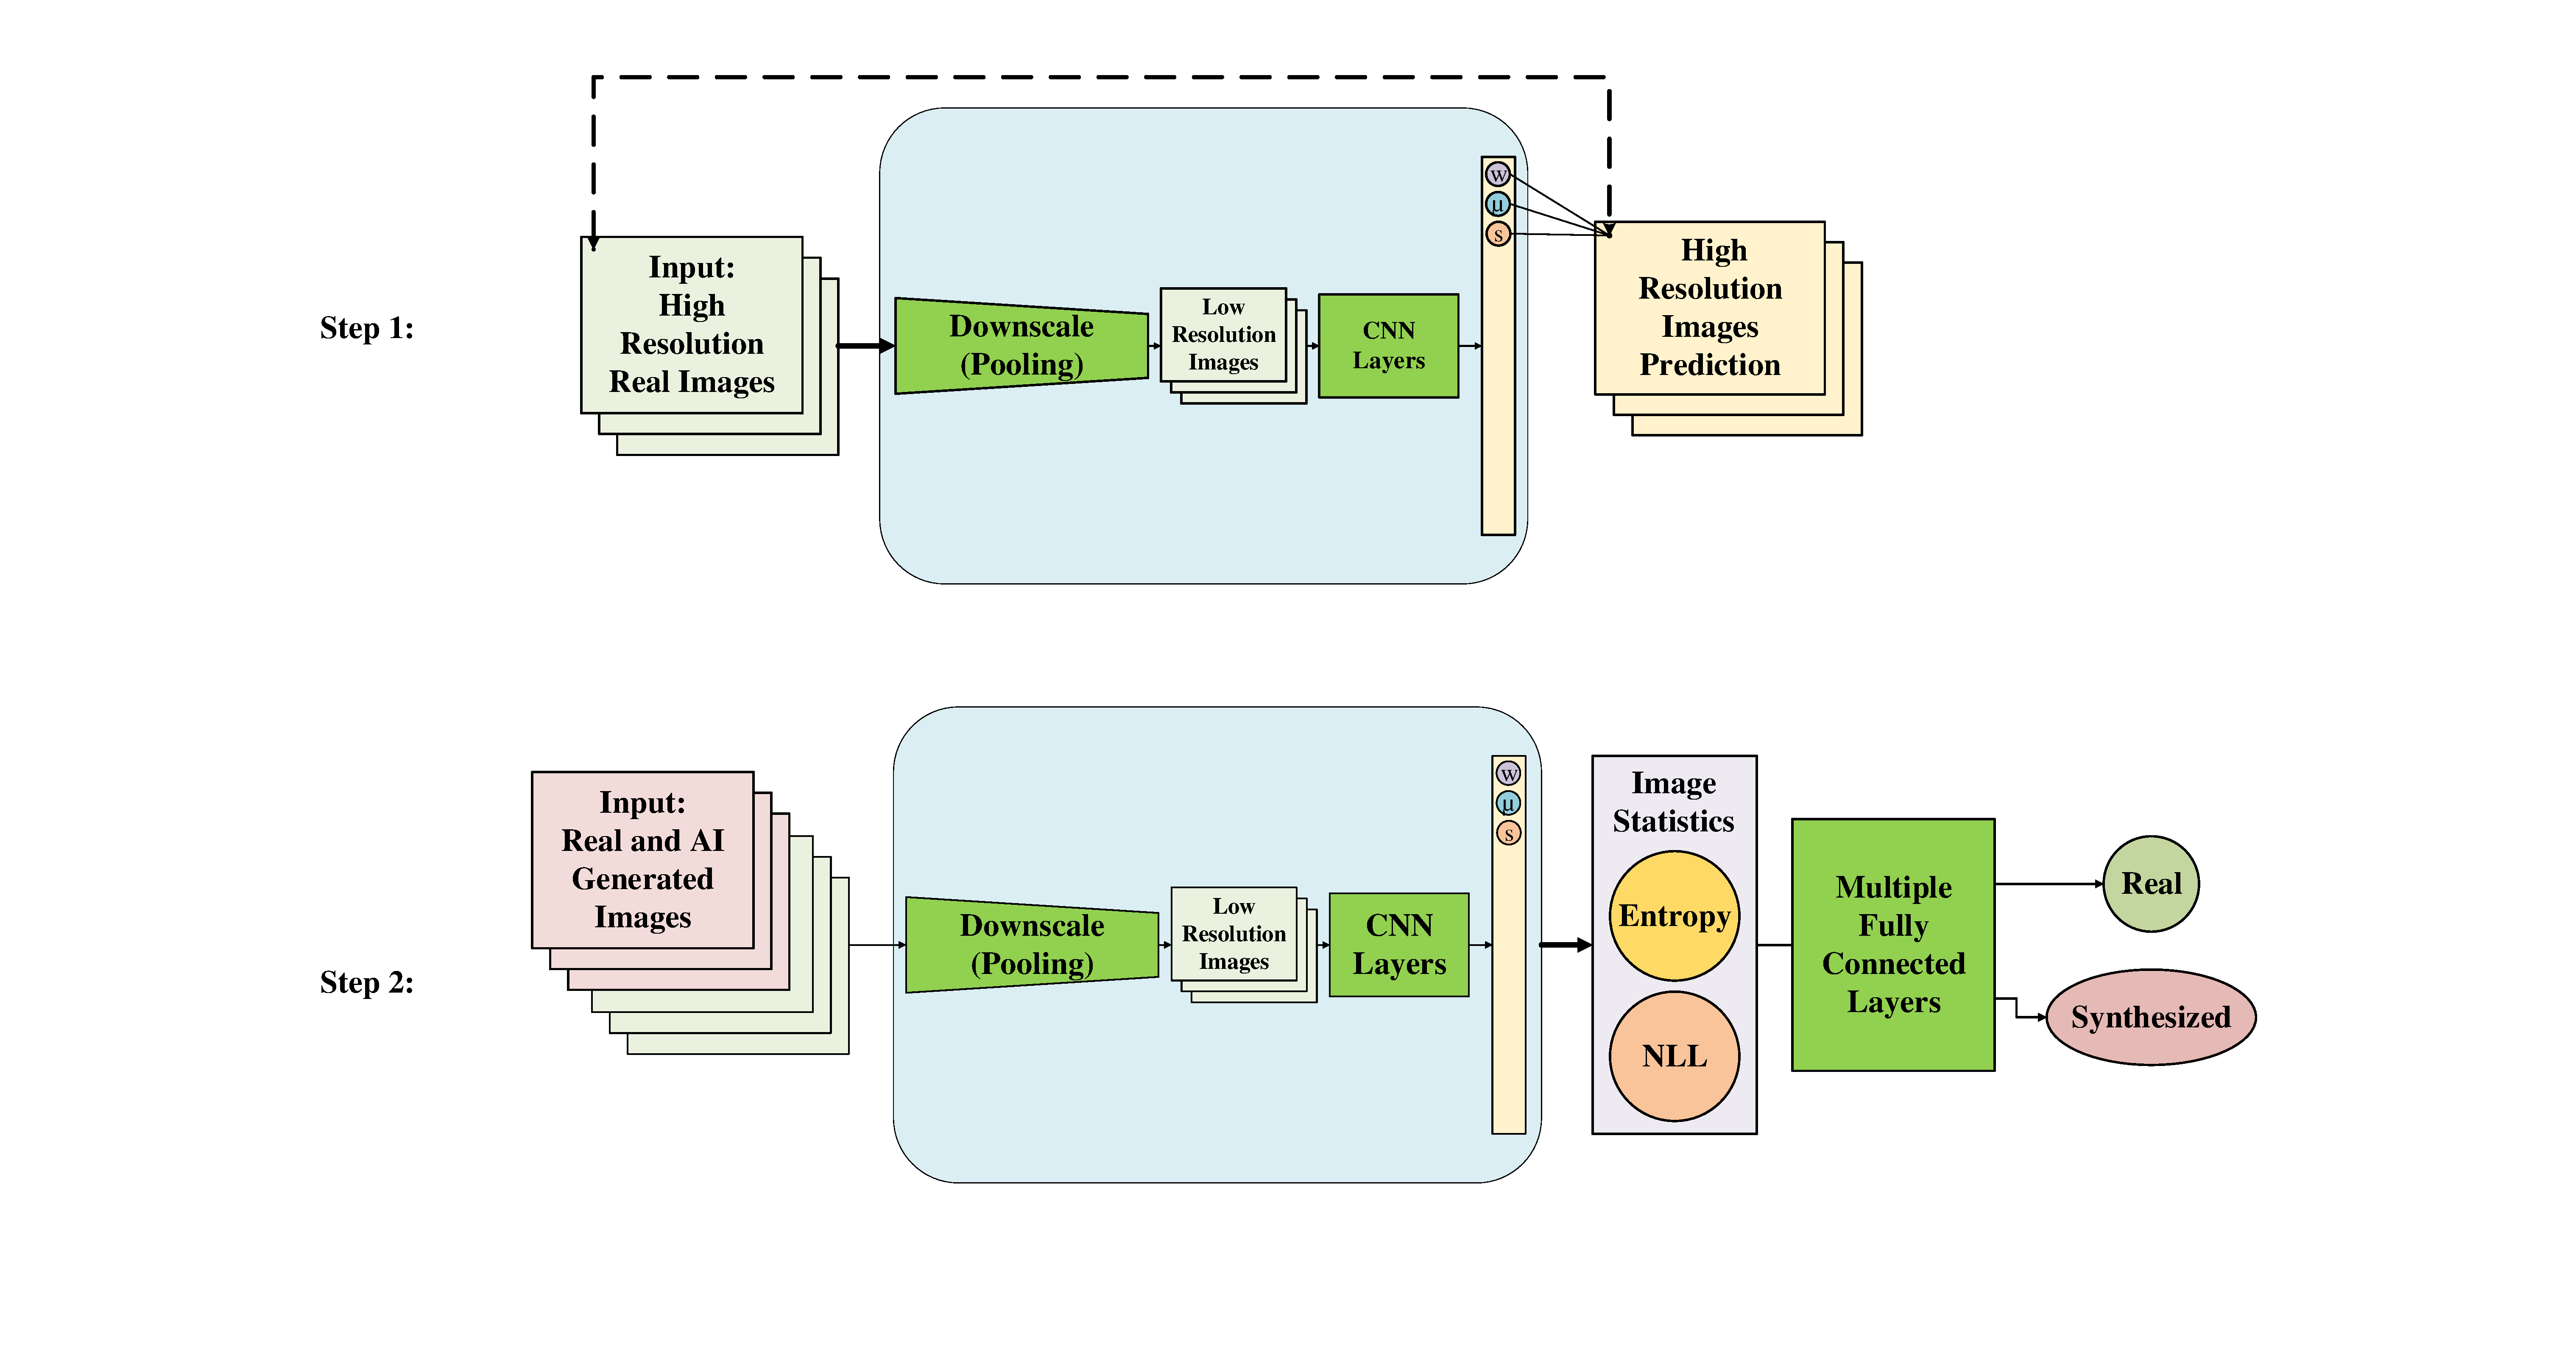
\includegraphics[width=\linewidth]{Fig/high_level_architecture.pdf}
    \caption{Two-step high level architecture for AI-generated image detection. Step 1 (top) trains a compression and reconstruction model (blue box) solely on real images, which downscales high-resolution images using an average pooling, and learn to reconstruct the high resolution image using CNN layers and logistic probability distribution parameters. Step 2 (bottom) applies the trained model (blue box) to both real and AI-generated images, extracting entropy-based statistics such as Negative Log-Likelihood (NLL) and entropy values. These statistics are passed through multiple fully connected layers for final classification.}
    \label{fig:high-level-architecture}
\end{figure}

\section{Background \& Related Work}
\label{background}

Image synthesis is the process wherein an artificial image is generated by a computer from an input prompt, which may be text or some other form of media. This field exploded after the creation of Generative Adversarial Networks (GAN) in 2014, a deep learning architecture particularly adept at generating photorealistic images \citep{GANfather}. More recently, diffusion models (DM) have also been a popular choice for image synthesis \citep{latent-diffusion}. While many attempts have been made to develop programs that can detect images generated by these architectures, they continually evolve to outsmart old detectors.

\subsection{Sightengine}

There are a number of AI-generated image detection websites which are free to use. One of these is \citet{sightengine}, which has a high accuracy rate compared to many other websites: approximately 99\% on real images and 81\% on AI-generated ones \citep{li2024adversarialaiartunderstandinggeneration}. However, it is far from foolproof. For example, when tested on images generated from image prompts by Dream Studio and DALL-E, its accuracy falls to only 34\%. As opposed to images generated from text promts, images generated from real image prompts may be more challenging to detect, since they are more likely to be very similar to the real images they were generated from.

Many free websites like sightengine also predict the source of AI-generated images among many commonly-used synthesis models. Although the accuracy of this feature has not been formally investigated, it seems to fail often.

Though sightengine has not published its methods for AI-generated image detection, there are a number of open-source detectors available online, some of which are discussed below.

\subsection{Beyond the Spectrum}

Many earlier attempts at AI-generated image detection focused on GAN-generated images, since using DMs for image synthesis only began in 2022. One of these is Beyond the Spectrum (BtS), an open-source project \citep{he2021spectrumdetectingdeepfakesresynthesis}.

Its method for detection involves two stages. First, a re-synthesizer is trained, only on real images, to reconstruct images from their downsampled versions. Next, this re-synthesizer is given both real and fake images, and the reconstruction error (which is assumed to be greater for GAN-generated images) is given to a classifier to predict whether a given image is real or not.

In 2021, BtS achieved approxiately 90\% accuracy on its testing datasets and was state-of-the-art (SoTA). However, in 2024, after the progression of GAN models and the advent of DMs, BtS achieves only a 21\% accuracy rate \citep{li2024adversarialaiartunderstandinggeneration}. Nonetheless, its approach is echoed in more recent successful approaches, such as the zero-shot method discussed in \ref{ZED}.

\subsection{Contrastive Language–Image Pretraining}

Another architecture that has been explored for detecting AI-generated images is Contrastive Language–Image Pretraining (CLIP), which was developed by OpenAI in 2021 \citep{radford2021learningtransferablevisualmodels}. This model is trained on pairs of images and text, and in the context of AI-generated image detection, this text might either be their prompts or human-written descriptions. CLIP was used to achieve an accuracy of 95-100\%, making it a promising model for AI-generated image detection \citep{moskowitz2024detectingaigeneratedimagesclip}.

\subsection{Vision Transformers}

In natural language processing, text is interpreted as a sequence of tokens from which subsequent tokens can be predicted. Vision transformers (ViT) take a similar approach. Images are broken down into non-overlapping sections, like tokens, which are sent into an encoder comprised of multi-head attention and feed-forward neural networks. The output of the encoder is then passed into an MLP which classifies the image; in our case, it predicts whether the image is real or fake. In April 2024, researchers combined CLIP and ViT (CLIP-ViT) and were able to outperform a number of SoTA detection methods with an average accuracy of 90\% \citep{cozzolino2024raisingbaraigeneratedimage}.

\subsection{Zero-Shot Entropy-Based Detector}
\label{ZED}

The main issue in designing AI-generated image detectors is that image synthesis models are constantly evolving to circumvent detectors trained on old data. In September 2024, a new zero-shot method was devised which initally only trains on real images \citep{cozzolino2024zeroshotdetectionaigeneratedimages}. First, a CNN is trained to predict real images from encoded versions of those images. Next, the CNN is used to predict both real and fake images from their encoded versions, and loss statistics used to differentiate real images from synthetic ones. Higher loss generally corresponds to AI-generated images, since the CNN provides a good model for real images.

This method was able to achieve an accuracy of 90\%, better than many other SoTA models. However, one drawback is that training and testing datasets were comprised only of uncompressed images.

\section{Data Processing}
\label{data}
Our model involves two phases of training (see \ref{arch}). As such, we require five datasets: two training sets, two validation sets, and one testing set. The first phase is trained only on real images, meaning that one training set and one validation set will be comprised only of real images. For the other training and validation sets, it is crucial to process data in order to minimize bias. We have identified the most potentially impactful bias in our data as being the semantic content of the images.

\subsection{Data Collection}
\label{data_coll}
% Suggestions (Nathan):
% Do the in-text citations for RAISE and Dresden
% "mentioned in detail later": reference the section
% Split into more paragraphs -> easier to read
% Create a table showing this information (sources, amounts, etc.) -> hard to keep track of numbers in sentences like this
To guarantee that the model is exposed to a diverse range of semantics, we will utilize two well-established camera-based digital forensics datasets: 1. RAISE: A Raw Images Dataset For Digital Image Forensics; 2.The 'Dresden Image Database' For Benchmarking Digital Image Forensics. These datasets collectively contain approximately 22,000 real images, captured under varying conditions and environments. The model will be trained in two phases which will be mentioned in detail later. For the first phase, 10,000 real images will be allocated for training and 2,000 real images for validation. For the second phase, 5,000 real images will be allocated for training and 1,000 images for validation. The remaining 2,000 real images will be reserved for evaluation in the testing phase. For the second phase, 5,000 synthetic images will also be used to training and 1,000 for validation which enables the model to develop a robust entropy-based understanding of real-world image statistics.
The testing dataset will be balanced, comprising 2,000 real images and 2,000 AI-generated images. The synthetic images will be sourced from the SyntheticEye AI-Generated Image Dataset [SyntheticEye Reference], which includes images produced by a range of state-of-the-art generative models, including Stable Diffusion, DALL-E, and others. Incorporating AI-generated images from multiple sources ensures that the testing conditions closely reflect real-world inputs, enhancing the model's ability to generalize across diverse synthetic image distributions.

\subsection{Data Modification}
\label{data_mod}
For image inputs, the CNN requires a fixed resolution of 256×256 pixels. To ensure compatibility, all images in both the training and testing datasets will be cropped to 256×256 while preserving their essential features.
Additionally, to prevent any biases arising from variations in image attributes, all datasets will be normalized and standardized. This includes converting all images to RGB color space, ensuring uniform channel distributions across the dataset. Standardizing the color format enhances consistency in feature representation, improving the model's robustness and generalization.

\section{Architecture}
\label{arch}
\subsection{Motivation}

Nowadays, image classification models typically use Convolutional Neural Networks (CNN) as their base architecture. Classical CNNs will use datasets that consists of AI-generated images to train and learn special attributes about these artificial pictures. But inefficiencies in the training process of CNNs are starting to surface as more and more image generation models are being released. With more image generation models come different characteristics that the CNN classifier never learned. This leads towards a need for training with the new datasets which both takes time and money (Cozzolino et al. 2024).

% Suggestion (Nathan):
% Nowadays, image classification models typically use Convolutional Neural Networks (CNN) as their base architecture. Classical CNNs train on datasets of AI-generated images to learn special features that are otherwise undetectable. However, as more and more image generation models are released, these CNNs are routinely oustmarted. New image generation models carry new characteristics which the CNN never learned. This creates a need for further training with new datasets, which takes both time and money (Cozzolino et al. 2024) PROPER CITATION.

% Nathan:
% We shouldn't use the name "Zero-Shot Entropy Detector". that is the name of the project from the paper and we shouldn't copy that I don't think. We can just talk about (a) zero-shot method(s). Also, only the first stage is zero-shot, just to be clear
The Zero-Shot Entropy Detector (ZED) is unique in a way that its training process for detecting AI-generated images doesn't rely on synthetic data sets. The main idea behind ZED is to estimate how ``surprising'' an image is compared to the real images it trained on. It is assumed that real images follow a ``natural'' statistic pattern, while AI-generated images typically consists of ``unnatural'' statistical patterns that are detectable \citep{cozzolino2024zeroshotdetectionaigeneratedimages}.

% entropy and nll based, so maybe it's image statistic based?
% we did used ai images in the second step training
% I think we need to mention nll entropy is enough to detemine if a image is ai generated from the zed paper
% Nathan:
% instead of entropy-based i think we can say loss-based, since we might pick slightly different decision stats. also it might not be clear what entropy is
% Reference William's figures
\subsection{Architecture}
\label{sec:architecture}

% Training the architecture of our neural network consists of two phases: (1) CNN training and (2) loss-based classification.
Our proposed model follows a two-step training process: (1) CNN treaing and (2) loss-based classification.

\subsubsection{Step 1: Real Image Compression and Reconstruction}
% In stage (1), WILLIAM ADD HERE the downsized versions of real images are given to a CNN as inputs. The CNN will upscale these images and predict their original full-sized versions.  
% Comments (Nathan):
% The model doesn't learn to downscale the images, I think this is just done through average pooling
% Use \ref{}s to reference your figure
The first step, illustrated in \ref{fig:high-level-architecture}, involves training an image compression and reconstruction model \textbf{solely on real images}. The model downscale and learns to reconstruct high-resolution images using pooling operations and convolutional layers (CNN). Specifically:
\begin{itemize}
    \item Real high-resolution images are downscaled through pooling layers and passed to a multi-layered CNN as inputs.
    \item The CNN extracts essential features and maps them to a latent space representation and upscale these images, and conects to a fully connected layer.
    \item The fully connected layer then predicts the \textbf{weight, mean, and scale} parameters for logistic probability distributions, which are used to reconstruct the original high-resolution image.
    \item The error between the predicted and expected output will be used to adjust the weights and biases of the CNN's filters through backpropagation.
\end{itemize}

This first stage is zero-shot, meaning it will not require retraining on synthetic data upon the advent of new image-generating AI models. And the CNN will be able to capture statistic features that only real images share. 

\subsubsection{Step 2: Real vs. AI-Generated Image Classification}
% Suggestion (Nathan):
% In stage (2), we no longer train the CNN, and it will provide a good model for upscaling real images, but not AI-generated ones. In this stage, we will give the CNN both real and generated images. We will calculate loss statistics on its output, and use these statistics as the input to a classifier. SOME CONCLUSION HERE
The second step, illustrated in \ref{fig:high-level-architecture}, the model is extended to classify images as real or AI-generated. This stage leverages both real and AI-generated datasets:
\begin{itemize}
    \item Input images, including both real and AI-generated high-resolution images, undergo the same compression and reconstruction process as in Step 1.
    \item Using the obtained \textbf{mean, weight, and scale} parameters, the model computes loss statistics such as \textbf{Negative Log-Likelihood (NLL) and entropy values and etc} for each image.
    \item These computed statistics are then passed through multiple fully connected layers to classify whether an image is real or AI-generated.
    \item Binary cross entropy from comparing with real and AI-generated labels will be used to train only the fully connected layers through backpropagation.
\end{itemize}

This second stage builds on top of CNN's ability to accurately reconstruct real images learned in the first step, and learns to utilize nuances between their loss statistic to perform classification. 


By structuring the model in this two-step process, we ensure that the first stage learns an accurate representation of natural image statistics, which the second stage leverages to effectively detect synthetic images.








\section{Baseline Model}
\label{baseline}

Our baseline model will mirror \citet{wang2020cnngeneratedimagessurprisinglyeasy}, an early attempt at AI-generated image detection. This model uses ResNet-50 trained on real images from ImageNet and fake images generated by three GAN architecures. We will expand our dataset to include fake images from a greater variety of image generators, including diffusion models (see \ref{data}).

We will not use ResNet-50 due to its complexity. Instead, we will implement our own ResNet-inspired 10-layer CNN as detailed in Table \ref{baseline_arch}.

    \begin{table}[t]
    \caption{Baseline model architecture: convolutional layers}
    \label{baseline_arch}
    \begin{center}
    \begin{tabular}{llllll}
    \multicolumn{1}{c}{\bf Convolution Layer}   & \multicolumn{1}{c}{\bf Kernel Size}   & \multicolumn{1}{c}{\bf Padding}    & \multicolumn{1}{c}{\bf Stride}   & \multicolumn{1}{c}{\bf Channels}   & \multicolumn{1}{c}{\bf Dimensions}
    \\ \hline \\
    Input               & N/A   & N/A   & N/A   & 3     & 256×256 \\
    Conv. 1             & 7×7   & 3     & 2     & 64    & 128×128 \\
    Average pooling     & 2×2   & 0     & 2     & 64    & 64×64 \\
    Conv. 2             & 3×3   & 1     & 1     & 64    & 64×64 \\
    Conv. 3             & 3×3   & 1     & 1     & 64    & 64×64 \\
    Conv. 4             & 3×3   & 1     & 2     & 128   & 32×32 \\
    Conv. 5             & 3×3   & 1     & 1     & 128   & 32×32 \\
    Conv. 6             & 3×3   & 1     & 2     & 256   & 16×16 \\
    Conv. 7             & 3×3   & 1     & 1     & 256   & 16×16 \\
    Conv. 8             & 3×3   & 1     & 2     & 512   & 8×8 \\
    Conv. 9             & 3×3   & 1     & 1     & 512   & 8×8 \\
    Average pooling     & 4×4   & 0     & 2     & 512   & 2×2 \\
    \end{tabular}
    \end{center}
    \end{table}

Notes:
\begin{itemize}
    \item We will create skip connections from the inputs to layers 2, 4, 6, and 8 to the outputs of layers 3, 5, 7, and 9, respectively.
    \item Skip connections with mismatched dimensions will be downsized using average pooling.
    \item The activation function for all convolutional layers will be ReLU.
    \item The output of the last average pooling layer will be a fully-connected layer with 2,048 neurons. These feed directly into the one-neuron output layer.
    \item The net will use a binary cross-entropy loss function.
    \item We will use the Adam optimizer with $\beta_1 = 0.9$ and $\beta_2=0.99$.
    \item We will train over 3,000 iterations.
    \item We will use learning rates of 0.01, 0.001, and 0.0001 for the first, second, and third sets of 1,000 training iterations, respectively.
\end{itemize}

\section{Ethical Considerations}
\label{ethical}

\subsection{Data Collection and Bias}
The implementation of AI-generated image detectors raises several ethical concerns, particularly regarding data collection and privacy. If the dataset used to train the detector contains personal or sensitive images, there is a risk of violating individuals' privacy rights. Additionally, the dataset may be biased, detecting AI-generated images only from certain architectures or sharing certain features while failing to generalize to others.

% Suggestion (Nathan): Maybe tie in better with data processing section? Ie. how will we do this
To minimize these risks, we ensure that our dataset is obtained from \textbf{peer-reviewed papers and licensed Kaggle datasets}. Furthermore, we use \textbf{balanced, diverse, and multi-source datasets} to reduce bias and avoid over-reliance on any single source, as stated in \ref{data_coll}.

\subsection{Misuse and Limitations}
The use of AI-generated image detectors also poses risks related to model accuracy and potential misuse. Due to the inherent uncertainty in AI models, achieving \textbf{perfect reliability} in distinguishing real and AI-generated images is generally infeasible, regardless of how well the model performs during testing. As a result, there is always a possibility of \textbf{false accusations}, where real images are mistakenly classified as AI-generated. The consequences of such misclassifications against legitimate artists can be severe and, in some case, irreversible. To mitigate this, we will explicitly \textbf{disclaim that the model is not 100\% accurate} and should be \textbf{used with caution}. It is meant to assist rather than serve as final proof in any legal or professional decisions.

By taking these measures, we aim to ensure that our AI tool is ethically sound, responsibly deployed, and used within appropriate legal boundaries.


\section{Project Plan}
\label{plan}

Team communication will be crucial to our success. Our main channel of communication will be a \textbf{Whatsapp group chat}, which we have used thus far. We will meet once \textbf{every Sunday at 10am}, but should we need to meet more frequently, we will use our chat to determine meeting times on a rolling basis.

To ensure team cohesion and clear delineation of tasks, we will (a) assign specific tasks to each team member as explained in \ref{assigning_work} and (b) use Git for version control.

\subsection{Assigning Work}
\label{assigning_work}

For written deliverables, we will all brainstorm ideas for each section. However, to ensure that we do not overwrite each other's work, each team member will be responsible for drafting certain sections. The point total of one member's assigned sections should be similar to the totals of every other team member's assigned sections to \textbf{ensure equal work}. We will use \textbf{Git for version control} so that we can clearly see the contributions of each team member. Using LaTeX comments, our group chat, and verbal communication, we will notify each other of suggestions that we have for each other's work.

Regarding work on the project itself, we will equally delineate ``substantial tasks'' as described in the Project Final Report Handout and Rubric (see \ref{detailed_plan}). This we will ensure that we are not overwriting each other's work and that we each share an equal load of the total work. Like with written deliverables, we will use comments, our group chat, and verbal communication to share suggestions for each other's work.

\subsection{Detailed Plan}
\label{detailed_plan}

Table \ref{plan_table} shows our internal deadlines for various components of the project throughout the rest of the semester. Though we will each work on all aspects of the projects, each aspect will be spearheaded by certain group members.

Description of tasks:
\begin{itemize}
        \item \textbf{Data Collection \& Verification:} Make a final determination on data sources, and add to GitHub respository.
        \item \textbf{Data Preprocessing:}              Split data into five sets as described in \ref{data_mod}. Ensure similar semantic content between real and fake images. 
        \item \textbf{Baseline Model Implementation:}   Implement and train model detailed in \ref{baseline}. Ensure non-random performance.
        \item \textbf{Primary Model Design:}            Implement and begin training on both stages of the architecture propoposed in \ref{arch}. Ensure performance is at least as good as the baseline.
        \item \textbf{Primary Model Training \& Optimization:} Finish training the primary model over multiple hyperparameters, and select the best model based on validation data.
        \item \textbf{Primary Model Analysis:}          Perform qualitative and quantitative analysis of the model on test data. Compare the efficacy of this model to the baseline model.
\end{itemize}

    \begin{table}[t]
    \caption{Project internal deadlines.}
    \label{plan_table}
    \begin{center}
    \begin{tabular}{llll}
    \multicolumn{1}{c}{\bf Task}            & \multicolumn{1}{c}{\bf Internal Deadline} & \multicolumn{1}{c}{\bf Task Lead(s)} & \multicolumn{1}{c}{\bf Status}
    \\ \hline \\
    Data Collection \& Verification         & 02-23                                     & Paul \& Vedansh       & In progress \\
    Data Preprocessing                      & 03-01                                     & Paul \& Vedansh       & Not started \\
    Baseline Model Implementation           & 03-01                                     & Nathan \& Paul        & Not started \\                   
    Primary Model Design                    & 03-16                                     & Nathan \& William     & Not started  \\
    Primary Model Training \& Optimization  & 03-25                                     & Nathan \& William     & Not started  \\
    Primary Model Analysis                  & 03-30                                     & Vedansh \& William    & Not started  \\
    \end{tabular}
    \end{center}
    \end{table}
    

\section{Risk Register}
\label{risk}
% no deep fake
Creating a successful AI-based generative image detection model involves various risks that may affect the project's outcome. This section highlights significant risks, evaluates their probability and effects, and presents detailed mitigation strategies.

\subsection{Insufficient Data Diversity}
\textbf{Likelihood:} Moderate \\
\textbf{Impact:} A lack of diverse training data can lead to a model that generalizes poorly to real-world scenarios, limiting its ability to detect AI generated fake images using different techniques or involving diverse demographics.

\textbf{Mitigation Strategies:}
\begin{itemize}
    \item \textbf{Data Augmentation:} Apply geometric transformations (e.g., rotation, scaling, flipping), color adjustments (e.g., brightness, contrast), and noise injection to artificially increase dataset variability \citep{shorten2019}. This will help the model adapt to various alterations typical in AI-generated images.
    \item \textbf{Continuous Data Acquisition:} Regularly update the dataset with newly generated AI images from emerging technologies to ensure that the model stays current and can detect the latest deep fake techniques.
\end{itemize}

\subsection{Prolonged Training Time}
\textbf{Likelihood:} High \\
\textbf{Impact:} Extended training times can delay project milestones, reduce iteration speed, and limit experimentation with different model architectures.

\textbf{Mitigation Strategies:}
\begin{itemize}
    \item \textbf{Transfer Learning:} Utilize pre-trained models like EfficientNet to reduce training time while maintaining high performance \citep{tan2019}. ResNet-based architectures, such as SRResNet, can enhance image resolution for better deep fake detection \citep{ledig2017}.
    \item \textbf{Cloud-Based GPU Resources:} Leverage high-performance computing resources through platforms such as Google Colab Pro, AWS SageMaker, and Microsoft Azure to accelerate training processes.
    \item \textbf{Optimized Code Practices:} Implement efficient data loading pipelines (using Optimized Data Storage), mixed-precision training (for weights and activations), and parallel processing to enhance computational efficiency.
\end{itemize}

\subsection{Overfitting}
\textbf{Likelihood:} Moderate \\
\textbf{Impact:} Overfitting results in a model that performs well on training data but poorly on unseen data, compromising its real-world effectiveness.

\textbf{Mitigation Strategies:}
\begin{itemize}
    \item \textbf{Regularization Techniques:} Apply dropout layers, L2 regularization, and batch normalization to prevent over-reliance on specific features \citep{srivastava2014}.
    \item \textbf{Cross-Validation:} Use k-fold cross-validation to ensure the model's robustness across different data splits, reducing the likelihood of overfitting to specific subsets.
    \item \textbf{Early Stopping:} Monitor validation loss during training and halt the process when performance plateaus or degrades, preventing unnecessary overfitting (stopping with patience).
\end{itemize}

\subsection{Technical Skill Gaps}
\textbf{Likelihood:} Moderate \\
\textbf{Impact:} Knowledge gaps in specific areas (e.g., advanced machine learning techniques, cloud computing) can slow down development and affect model performance.

\textbf{Mitigation Strategies:}
\begin{itemize}
    \item \textbf{Skill Development:} Leverage online courses (e.g., Coursera) and organize group study sessions to address specific knowledge gaps.
    \item \textbf{Mentorship:} Seek advice from professors, TAs, or online platforms like Stack Overflow and GitHub for problem-solving support.
    \item \textbf{Task Allocation:} Distribute tasks based on each team member's strengths to optimize efficiency and project quality.
    \item \textbf{Scoping:} If knowledge gaps are too large, refine the project scope to align with the team's current skill level, ensuring the project remains achievable within the timeline.
\end{itemize}

\subsection{Model Underperformance}
\textbf{Likelihood:} Moderate \\
\textbf{Impact:} An underperforming model may fail to detect fake AI generated images from real ones with high accuracy, reducing the system's reliability.

\textbf{Mitigation Strategies:}
\begin{itemize}
    \item \textbf{Architecture Refinement:} Experiment with different CNN architectures to optimize feature extraction from general images. Increase comlexity, number of layers, and number of parameters in the model.
    \item \textbf{Hyperparameter Tuning:} Use automated techniques like grid search, random search, or Bayesian optimization to fine-tune CNN parameters for optimal performance \citep{bergstra2011}.
\end{itemize}

\section{Link to GitHub}
The project's GitHub repository can be accessed at:  
\href{https://github.com/WilliamJWen/Project42}{https://github.com/WilliamJWen/Project42}


\label{last_page}

\bibliography{APS360_ref}
\bibliographystyle{iclr2022_conference}

\end{document}
